\documentclass[english]{article}
\usepackage[T1]{fontenc}
\usepackage[latin9]{inputenc}
\usepackage{textcomp}
\usepackage{amsmath, amsfonts}
\usepackage{babel}
\usepackage{lscape}
\makeatletter
\@ifpackageloaded{tex4ht}{%
  \def\pgfsysdriver{pgfsys-tex4ht.def}%
}{%
  % only needed inside a class
  \begingroup\expandafter\expandafter\expandafter\endgroup
  \expandafter\ifx\csname HCode\endcsname\relax
  \else
    \def\pgfsysdriver{pgfsys-tex4ht.def}%
  \fi
}
\makeatother


\title{SixTrackLib Manual}
\author{R. De Maria, M. Fitterer, M. Fjellstrom, P. Hermes }


\usepackage{tikz}
\usetikzlibrary{3d,calc}
\usepackage{cite}
\usepackage{url}

\DeclareMathOperator{\sgn}{sgn}
\DeclareMathOperator{\erf}{erf}

\tikzset{math3d/.style= {x={(1cm,0cm)}, y={(0.353cm,0.353cm)}, z={(0cm,1cm)}}}

\def\PD#1#2{\frac{\partial #1}{\partial #2}}
\def\TD#1#2{\frac{d #1}{d #2}}
\def\PnD#1#2#3{\frac{\partial^{#3} #1}{\partial #2^{#3}}}
\def\TnD#1#2#3{\frac{d^{#3} #1}{d #2^{#3}}}




\begin{document}
  \maketitle 
  
  


\section{Introduction}

These notes give a short self-contained exposition of the physical assumptions
and models implemented in SixTrack. Emphasis is given on the physical concepts
rather then delving in to the details of the implementation.  The content is
meant to complement the SixTrack user guide (see \cite{user_guide}).

SixTrack is a 6D single particle symplectic tracking code used to compute the
trajectories of individual relativistic charged particles in circular
accelerators. It has been developed based on the 4D tracking code RaceTrack
\cite{racetrack} by adding the third degree of freedom, introducing beam-beam
forces and extending the pre- and post- processing capabilities.

The physical models are collected from the main references
\cite{ripken85,barber87,ripken95,heinemann95,barber96,beam_beam,rf_multipoles},
which contain more details of the derivation of the maps.


\section{Reference frame}

The speed, momentum, energy, rest mass, charge of a particle are indicated
by $v$, $P$, $E$, $m$ and $q$, respectively.  These quantities are
related by the following equations:
\begin{align}
  v&=\beta c &
  E^2-P^2c^2&=m^2c^4 &
  E & = \gamma mc^2 &
  Pc & =\beta E
\end{align}
where $\beta$ and $\gamma$ are the relativistic factors.

In a curvilinear reference frame defined by a constant curvature $h_x$ in the
$\hat X, \hat Z$ plane and parameterized by $s$  (see Fig. \ref{fig:frame}), the
position of the particle at a time $t$ can be written as:
\begin{align}
  \vec Q(t)= \vec r(s) + x \,\hat x(s) + y\, \hat y(s),
\end{align}
and therefore identified by the coordinates $s, x, y, t$ in the reference frame
defined by $\hat x(s)$ and $\hat y(s)$. In particle tracking, $s$ is normally
used as independent parameter and $t$ as a coordinate.

The electromagnetic fields {\bf E} and {\bf B} can be derived in a curvilinear
reference frame from the potentials $V(x,y,s,t)$ and $\mathbf{A}(x,y,s,t)$, where
\begin{align}
\mathbf{A}(x,y,s,t)=A_x(x,y,s,t) \hat x(s) + A_y(x,y,s,t) \hat y(s) + A_s(x,y,s,t) \hat z(s)
\end{align}
and for which:
\begin{align}
  \mathbf{E}  &= -\nabla V - \frac{\partial \mathbf{A}}{\partial t} 
               = -\partial_x V \hat x - \partial_y V \hat y -
  \frac{1}{1+h x}  \partial_s V \hat z - \partial_t \mathbf{A}\\
  \mathbf{B} &= \nabla\times\mathbf{A}  =
  \left(\partial_y A_s - \frac{\partial_s  A_y}{1+h x} \right) \hat x 
  +\left(\frac{\partial_s A_x-\partial_x (1+h x) A_s }{1+h x} \right)\hat y \\
  &+\quad \left(\partial_x A_y - \partial_y A_x \right) \hat z.
\end{align}
In this reference frame the canonical momenta are:
\begin{align}
  P_x&=m \gamma \dot x + q A_x, &
  P_y&=m \gamma \dot y + q A_y, &
  P_s&=m \gamma \dot s (1 + h x)^2 + q (1 + h x) A_s.
\end{align}
and the energy of a particle and the field is
\begin{align}
E=qV + c \sqrt{(mc)^2
              +\frac{(P_s- q A_s(1+hx))^2}{(1+hx)^2}
              +(P_x-q A_x)^2 + (P_x-q A_x)^2}.
\end{align}







\section{Hamiltonian}

If $s(t)$ is monotonically increasing, it is possible to derive the equations
of motion using $s$ as the independent parameter and $t$ as a coordinate with
$-E$ as the conjugate momentum by using $P_s$ as Hamiltonian.

\begin{align}
  P_s&= (1+h x) \left( 
       \sqrt{ E^2 - (mc^2)^2
           - (P_x - q A_x)^2
           - (P_y - q A_y)^2}
       +q A_s
    \right)
\end{align}

Since in accelerators the orbits of the 
particles are often a perturbation of the reference trajectory followed by a
particle with rest mass $m_0$, charge $q_0$, speed $\beta_0 c$ and momentum
$P_0$, one could use the following derived quantities that usually assume small
values


\begin{align}
p(x,y) &= \frac{m_0}{m}\frac{P(x,y)}{P_0}   &
\chi &= \frac{q}{q_0}\frac{m_0}{m} &
a(x,y,s) &= \frac{q_0}{P_0}  A(x,y,s) \\
\delta &= \frac{P \frac{m_0}{m} -P_0}{P_0} &
p_t &= \frac{E \frac{m_0}{m} -E_0}{P_0c} &
p_\sigma &= \frac{E \frac{m_0}{m} -E_0}{\beta_0 P_0c}
\\
\Delta s &= s - \beta c t &
\tau &= \frac{s}{\beta_0} - ct &
\sigma &= s - \beta_0 ct &
\end{align}

and redefine the Hamiltonian by:

\begin{align}
 H_\tau   &= \frac{p_t}{\beta_0} - \frac{m_0}{m}\frac{P_s}{P_0} &
 H_\sigma &= p_\sigma - \frac{m_0}{m}\frac{P_s}{P_0}
\end{align}

\begin{align} 
 H_\tau   &= \frac{p_t}{\beta_0} - (1+h x) \left(
      \sqrt{ (1+\delta)^2
           - (p_x - \chi a_x)^2
           - (p_y - \chi a_y)^2}
       + \chi a_s
    \right) \\
  H_\sigma &= p_\sigma - (1+h x) \left(
      \sqrt{ (1+\delta)^2
           - (p_x - \chi a_x)^2
           - (p_y - \chi a_y)^2}
       + \chi a_s
    \right),
\end{align}
where 
\begin{align}
\delta &= \frac{P \frac{m_0}{m} -P_0}{P_0} &
\chi &= \frac{q}{q_0}\frac{m_0}{m}.
\end{align}

The following identities are useful to derive the equation of motion.

\begin{align}
\delta&=\sqrt{p_t^2 + 2 p_t/\beta_0 +1} -1 &
\frac{d \delta}{d p_t}= \frac{p_t+1/\beta_0}{1+\delta} = \frac{1}{\beta} \\
\delta&=\sqrt{\beta_0^2 p_\sigma^2 + 2 p_\sigma +1} -1 &
\frac{d \delta}{d p_\sigma}= \frac{p_\sigma\beta_0^2+1}{1+\delta} = \frac{\beta_0}{\beta}
\end{align}


\section{Straight Drift}
A drift is a straight, field-free region ($h(x,y)=0$, $V=0$ and
$\mathbf{A}=0$).  The exact and expanded Hamiltonian for a drift space are
\begin{align}
  H_\tau = \frac{p_t}{\beta_0} - \sqrt{(1+\delta)^2 - p_x^2 - p_y^2} &\approx
  \frac{p_t}{\beta_0} - \delta + \frac{1}{2}\frac{p_x^2+p_y^2}{1+\delta}.
\end{align}
\begin{align}
  H_\sigma = p_\sigma - \sqrt{(1+\delta)^2 - p_x^2 - p_y^2} &\approx
  p_\sigma - \delta + \frac{1}{2}\frac{p_x^2+p_y^2}{1+\delta}.
\end{align}




\subsection{Expanded Drift}

The map relative to the expanded Hamiltonian is (eq. 3.49 in \cite{ripken95})
\begin{align}
  x_p &= \frac{p_x}{1+\delta} & 
  y_p &= \frac{p_y}{1+\delta}  \\
  x & \leftarrow x + x_p l &
  y & \leftarrow y + y_p l
\end{align}
\begin{align}
  \tau & \leftarrow \tau +
   \frac{l}{\beta_0} - \frac{l}{\beta} -
    \frac{l}{\beta} \frac{x_p^2+y_p^2}{2}=
    \tau+
    l\left(\frac{\delta}{\beta_0}-\frac{p_t}{1+\delta} - \frac{x_p^2+y_p^2}{2\beta}\right)
\end{align}
\begin{align}
  \sigma & \leftarrow \sigma +
   l - \frac{\beta_0}{\beta} l -
    \frac{\beta_0}{\beta} l \frac{x_p^2+y_p^2}{2}=
    \sigma+
    l\left(1- \frac{\beta_0}{\beta}\left(1 + \frac{x_p^2+y_p^2}{2}\right)\right)
\end{align}

\subsection{Exact Drift}

The map relative to the exact Hamiltonian is (eq. 3.49 in \cite{ripken95})
\begin{align}
  p_z&=\sqrt{(1+\delta)^2 - p_x^2 - p_y^2} \\
  \frac{d p_z}{d p_t}&= \frac{p_t+1/\beta_0}{p_z} = \frac{1}{\beta_z}  \\
  \frac{d p_z}{d p_\sigma}&= \frac{\beta_0^2 p_\sigma+1}{p_z} = \frac{\beta_0}{\beta_z}  
\end{align}
\begin{align}
  x & \leftarrow x + \frac{p_x}{p_z} l  &
  y & \leftarrow y + \frac{p_x}{p_z} l
\end{align}
\begin{align}
  \tau & \leftarrow \tau + \frac{l}{\beta_0}
  -\frac{l}{\beta_z}=
  l\left(\frac{1}{\beta_0}-\frac{p_t+1/\beta_0}{p_z}\right)
\end{align}
\begin{align}
  \sigma & \leftarrow \sigma + l
  -l \frac{\beta_0}{\beta_z}=
  l\left(1-\frac{\beta_0^2 p_\sigma+1}{p_z}\right)
\end{align}




\section{Polar Drift}
It is possible to define a ``polar'' drift that has the effect of rotating the reference frame
\cite{forest99} for instance in the $x$-$z$ plane

\begin{align}
p_x & \leftarrow   p_x \cos \theta + p_z \sin\theta &
p_z & \leftarrow - p_x \sin \theta + p_z \cos\theta \\
z   &= -x \sin \theta & x' &= p_x/p_z &  y' &= p_y/p_z \\
x   & \leftarrow x \cos\theta - x' z  &
y   & \leftarrow y - x' z  & \tau & \leftarrow \tau + z/\beta_z .
\end{align}
where $\theta$ is the angle bringing the new $\hat x$ towards the old $\hat z$.
The map can be also generated by combining a rotation with a $-x
\sin(\theta)$-length drift. In case of an $\hat x$ rotation the role of $x$ and $y$ are interchanged. 


\section{Dipole}

In a curvilinear reference system with a constant curvature $h$ in the
horizontal plane a uniform magnetic field can be derived by the vector potential:
\begin{align}
  A_x & = 0, & A_y & = 0, & A_s & = 
  - B_y \left(x-\frac{h x^2}{2 (1+h x)}\right).
\end{align}

With the following normalization $k_0=\frac{q_0}{p} B_y$ is the inverse of the bending 
radius of the reference particle.

The exact and expanded Hamiltonian for a horizontal bending magnet is (eq. 2.12 in
\cite{barber87})
\begin{align}
  H &= \frac{p_t}{\beta_0} 
       - (1+h x)\sqrt{(1+\delta)^2 -p_x^2 - p_y^2}
       + \chi k_0 \left( x + \frac{h x^2}{2} \right)  \\
    &\simeq   \frac{p_t}{\beta_0}
    + \frac{1}{2}\frac{p_x^2+p_y^2}{1+\delta}
  - (1+h x) (1+\delta) + \chi k_0 \left( x + \frac{h x^2}{2} \right)
\end{align}


\subsubsection{Thin dipole}
The map for a thin dipole kick (horizontal or vertical) from the expanded Hamiltonian is 
(eq. 4.12 in \cite{heinemann95}):
\begin{align}
  p_x &\leftarrow p_x + (h_x l - \chi k_0 l)  + h_x l \delta - \chi k_0 l h_x x \\
  p_y &\leftarrow p_y - (h_y l - \chi \hat k_0 l) - h_y l \delta + \chi k_0 l h_y y\\
  \tau &\leftarrow \tau - \frac{h_xx - h_yy}{\beta}  l.
\end{align}

\subsubsection{mad thin dipole}

to be checked
%??? dipr 
\begin{align}
  p_x &\leftarrow p_x + (h_x l - \chi k_0 l)  + h_x l (p_z -1) - \chi k_0 l h_x x \\
  p_y &\leftarrow p_y - (h_y l - \chi \hat k_0 l) - h_y l (p_z-1) + \chi k_0 l h_y y\\
  \tau &\leftarrow \tau - \frac{h_xx - h_yy}{\beta_z}  l.
\end{align}


 %   track(2,jtrk) = track(2,jtrk) - (dbr + dxt(jtrk) - dipr * (ttt - one))
 %    track(4,jtrk) = track(4,jtrk) + (dbi + dyt(jtrk) - dipi * (ttt - one))
 %    track(5,jtrk) = track(5,jtrk) - &
 %         (dipr*track(1,jtrk) - dipi*track(3,jtrk)) *   &
 %         ((one + bet0*track(6,jtrk))/ttt) * bet0i



\subsubsection{Thick dipole}
Defining the following quantities,
\begin{align}
  G_x&= \chi \frac{k_0 h_x}{1+\delta}, & G_y&= \chi \frac{ \hat k_0 h_y}{1+\delta} \\
  C_{x,y}&=\cos(\sqrt{G_{x,y}}L), & S_{x,y}&=\sin(\sqrt{G_{x,y}}L)
\end{align}
the map relative to the expanded Hamiltonian is (eq. 4.11 in \cite{barber87})
\begin{align}
  x   &\leftarrow C_x \cdot x + \frac{S_x}{\sqrt{G_x}}\frac{1}{1+\delta} \cdot p_x + \frac{\delta}{h_x} (1 - C_x) \\
  p_x &\leftarrow -\sqrt{G_x} (1+\delta) \cdot S_x \cdot x + C_x \cdot p_x + \delta \sqrt{1+\delta} \cdot S_x \\
  y   &\leftarrow C_y \cdot y + \frac{S_y}{\sqrt{G_y}}\frac{1}{1+\delta} \cdot p_y + \frac{\delta}{h_y} (1 - C_y) \\
  p_y &\leftarrow -\sqrt{G_y} (1+\delta) \cdot S_y \cdot y + C_y \cdot p_y + \delta \sqrt{1+\delta} \cdot S_y \\
  \sigma &\leftarrow \sigma + L\left(1 - \frac{\beta_0}{\beta}\right) \\
  & \qquad\, -\frac{\beta_0}{\beta} \Bigg[ \frac{h_x S_x}{\sqrt{G_x}} \cdot x + \frac{1-C_x}{h_x} \cdot p_x
  + \frac{h_y S_y}{\sqrt{G_y}} \cdot y + \frac{1-C_y}{h_y} \cdot p_y
  + \delta \left(2L - \frac{S_x}{\sqrt{G_x}} - \frac{S_y}{\sqrt{G_y}} \right) \Bigg] \\
  & \qquad\, - \frac{1}{4}\frac{\beta_0}{\beta} \Bigg[ G_x \left(L-\frac{C_xS_x}{\sqrt{G_x}} \right)
  \left(x - \frac{\delta}{h_x}\right)^2
  + \left(L+\frac{C_xS_x}{\sqrt{G_x}} \right) \frac{p_x^2}{(1+\delta)^2}
  -\left(x-\frac{\delta}{h_x}\right) \frac{2S_x^2}{1+\delta} \cdot p_x \\
  & \qquad\, + G_y \left(L-\frac{C_yS_y}{\sqrt{G_y}} \right)
  \left(y - \frac{\delta}{h_y}\right)^2 + \left(L+\frac{C_yS_y}{\sqrt{G_y}}\right) 
  \frac{p_y^2}{(1+\delta)^2}
  -\left(y-\frac{\delta}{h_y}\right)\frac{2S_y^2}{1+\delta} \cdot p_y \Bigg].
\end{align}

\subsubsection{Dipole Edge effects}
Considering the dipole edge effects from a dipole of length $L$ and bending angle $\theta$, 
the map is
\begin{align*}
    p_x &\to p_x + \frac{1+\delta}{\rho} \tan(\alpha) \cdot x \\
    p_y &\to p_y - \frac{1+\delta}{\rho} \tan(\alpha) \cdot y,
\end{align*}
where the bending radius $\rho$ and $\alpha$ are defined as
\begin{align*}
    \rho^{-1}   &= \frac{h_x}{\sqrt{1+\delta}} &
    \alpha &= \frac{1}{2} \frac{L}{\rho} = \frac{\theta}{2}.
\end{align*}




\section{Combined dipole quadrupole}

The following vector potential in curvilinear coordinates
\begin{align}
A_s= -\frac{g}{1+h x}
    \left(\frac{x^2}{2} - \frac{y^2}{2} +
          \frac{h x^3}{3} \right)
\end{align}
produce a field 
\begin{align}
B_x&= g \left(y + \frac{h x y}{1+h x} \right) &
B_y&= g x 
\end{align}

The following vector potential in curvilinear coordinates
\begin{align}
A_s= -\frac{g}{1+h x}
    \left(\frac{x^2}{2} - \frac{y^2}{2} +
          \frac{h x^3}{3} -   \frac{h x y^2}{2} \right)
\end{align}
produce a field 
\begin{align}
B_x&= g y &
B_y&= g \left(x + \frac{h y^2}{2+2 h x} \right) 
\end{align}


\section{Thin Multipole}

The effect of a thin multipole can be approximated by the following Hamiltonian

A longitudinally uniform static magnetic field can be described by the following equations
\begin{align}
    B_y+iB_x&=\sum_{n=1}     \frac{B_n+iA_n}{r_0^{n-1}} (x+iy)^{n-1} \\
            &=B_N \sum_{n=N} \frac{b_n+ia_n}{r_0^{n-1}} (x+iy)^{n-1}  .
\end{align}

Usually multipole are expressed as relative to 

A thin multiple idealize the effect of the field by taking the limit of the integration 
length going to zero while keeping constant the integrated strength. The Hamiltonian is:
\begin{align}
  H=- \delta(s) \chi l \Re\left[\sum_{n=0} (k_n + i\hat k_n) (x+iy)^{n+1} \right].
\end{align}
where
\begin{align}
  k_n     &=  n!\frac{q_0}{p_0}  \frac{B_{n+1}}{r_0^n}  &
  \hat k_n&=  n!\frac{q_0}{p_0}  \frac{A_{n+1}}{r_0^n} .
\end{align}


The corresponding map is:
\begin{align}
  p_x &\leftarrow p_x - \chi L\cdot\Re\left[\sum_{n=0} \frac{1}{n!} (k_n + i\hat k_n) (x+iy)^n \right], \\
  p_y &\leftarrow p_y + \chi L\cdot\Im\left[\sum_{n=0} \frac{1}{n!} (k_n + i\hat k_n) (x+iy)^n \right],
\end{align}

In case a curvature $h$ is the vector potential become:

\begin{align}
f(x,y)&=\int B_x(x,y) dy  \\
g(x,y)&=\int \partial x  B_x(x,y) dy \\
a_s(x,y)&=\frac{c_1}{1 + h x} + f(x,y) -
   \frac{\int_1^x (1 + h \xi) (g(\xi,y)+\xi) +h f(x,y)  \, d\xi}{1+ h x}
\end{align}

\begin{align}
\frac{\int_1^x \left(-h \xi \left(g(x,y)\right)-\int \text{bx}^{(1,0)}(\xi,y) \, dy-h \int \text{bx}(\xi,y) \,
   dy-h \xi \text{by}(\xi,y)-\text{by}(\xi,y)\right) \, d\xi}{h x+1}
\end{align}



\section{Accelerating Cavity}

The approximated energy gain of a particle passing through an electric field of frequency $f=\frac{k}{2\pi c}$ for which:
\begin{align}
V \sin(\phi - k \tau) = \int_{-l/2}^{l/2} E_s(0,0,t,s)  {\rm \,d}s.
\end{align}

An equivalent vector potential can be derived and normalized as
\begin{align}
A_s& = - \frac{V}{\omega} \cos(\phi - k \tau ) & 
V_n&=  \frac{q_0}{P_0 c} V  & 
\end{align}
from which one can derive the following map
\begin{align}
p_t & \leftarrow p_t + \chi V_n \sin(\phi - k \tau + k \frac{s-s_0}{\beta_0}  ),
\end{align}
where the additional terms in the phase is added in case harmonic number is not exactly integer and the phase is unlocked phase ). The new $\delta$ can be updated from the new $p_t$.



\section{RF-Multipole}

The RF-multipole generalizes the interaction of a particle with an electromagnetic field by assuming that

\begin{align}
\Delta E(x,y,\tau) &= q \int_{-L/2}^{L/2} E_z(x,y,t)  {\rm \,d}s \\
\Delta P_x(x,y,\tau) &= q \int_{-L/2}^{L/2} E_x(x,y,t) + \beta c B_y(x,y,t) {\rm \,d}s\\
\Delta P_y(x,y,\tau) &= q \int_{-L/2}^{L/2} E_y(x,y,t) - \beta c B_x(x,y,t) {\rm \,d}s.
\end{align}
are harmonic in $x,y$ and periodic in $\tau$ of frequency $f=\frac{k}{2\pi c}$ such that:

\begin{align}
a_s(x,y,\tau) 
&= \Re \left[ \sum_{n=1}^N
      \left(       k_n \cos(\phi_n -k \tau ) +
            i \hat k_n \cos(\hat \phi_n -k \tau)
      \right)    
      (x+i y )^n
     \right],
\end{align}

The map then follows:
\begin{align}
    \Delta p_x &= -\sum_{n=1}^N \frac{\chi}{n!} \Re\left[ (k_n C_n + i \hat k_n \hat C_n)(x+iy)^{(n-1)}\right], \\
    \Delta p_y &=  \sum_{n=1}^N \frac{\chi}{n!} \Im\left[ (k_n C_n + i \hat k_n \hat C_n)(x+iy)^{(n-1)}\right], \\
    \Delta p_t &= -\chi k \sum_{n=1}^N \Re\left[( k_n S_n + i k_n \hat S_n ) (x+iy)^n\right],
\end{align}
where
\begin{align}
     C_n&=\cos(\phi_n-\omega \Delta t) &
\hat C_n&=\cos(\hat \phi_n-\omega \Delta t) \\
     S_n&=\sin(\phi_n-\omega \Delta t) &
\hat S_n&=\sin(\hat \phi_n-\omega \Delta t) .
\end{align}


\section{Solenoid}
The expanded Hamiltonian for a particle in a solenoid is
\begin{align*}
  H &= p_\sigma+\frac{1}{2}\frac{(p_x+R\cdot y)^2+(p_y-R\cdot x)}{1+\delta},
\end{align*}
where $R=\frac{1}{2}\frac{q}{P_0c}\mathbf{B}(0,0,s)$. The map for a solenoid 
of length $L$ in the thin lens approximation with the expanded 
Hamiltonian (eq. 4.35 in \cite{heinemann95})
\begin{align*}
  x   &\to \,\,\,\,\, C\cdot x + S\cdot y \\
  p_x &\to -\theta R\cdot C \cdot x+C\cdot p_x
        -\theta R\cdot S\cdot y+S\cdot p_y \\
  y   &\to -S\cdot x + C\cdot y \\
  p_y &\to \,\,\,\,\, \theta R\cdot S\cdot x - S\cdot p_x 
  - \theta R\cdot C \cdot y + C\cdot p_y \\
  \sigma &\to \sigma - \frac{\beta_0}{\beta}
  \frac{\theta}{1+\delta} \left(\frac{1}{2}
  R (x^2 + y^2) + (p_xy - p_yx)\right)
\end{align*}
where $R\equiv R(s_0)$, $\theta=\frac{R}{1+\delta}$, 
$C=\cos(\theta)$ and $S=\sin(\theta)$.\\[0.5em]
The map for a thick solenoid is (eq. 3.47, 3.48 in \cite{ripken85}) 
\begin{align*}
    x &\to C^2 \cdot x+\frac{1}{R}\cdot S\cdot C\cdot p_x+S\cdot C\cdot y
    + \frac{1}{R}\cdot S^2 \cdot p_y \\
    p_x &\to -R\cdot S\cdot C\cdot x + C^2\cdot p_x
    -R\cdot S^2\cdot y + S\cdot C\cdot p_y \\
    y &\to -S\cdot C\cdot x -\frac{1}{R}\cdot S^2 \cdot p_x
    +C^2\cdot y + \frac{1}{R}\cdot S\cdot C\cdot p_y \\
    p_y &\to R\cdot S^2\cdot x -S\cdot C\cdot p_x
    -R\cdot S\cdot C\cdot y + C^2\cdot p_y \\
    \sigma &\to \sigma - \frac{L}{2} \left[R^2(x^2+y^2)+2R\left(
    \frac{p_x}{1+\delta}y - \frac{p_y}{1+\delta}x\right) 
    + \frac{p_x^2+p_y^2}{(1+\delta)^2} \right]
\end{align*}
where $\theta=R\cdot L$, $C=\cos\theta$ and $S=\sin\theta$.


\section{Beam-Beam}

The closed expression of an integrated kick experienced by a test particle of charge  $q=Z e$ due to a 2D uncoupled Gaussian charge distribution of total charge $q_b=N_b e$ defined by $\sigma_x, \sigma_y$ and located at $\Delta x, \Delta y$ from the test particle and moving at $v_z=\beta_b c$ from the test particle can be obtained through the use of complex the function \cite{bassetti-erskine}:

\begin{align}
w(z)=\exp({-z^2})\left(1+\frac{2i}{\sqrt{\pi}}\int_0^z \exp({\xi^2}) d\xi \right)=
     \exp({-z^2}){\rm erfc}(-iz).
\end{align}

The kick can then be expressed as
\begin{equation}
\Delta p_y+i \Delta p_x= K_b \frac{\sqrt{\pi}}{r}
\left( {\rm w}\left(\xi_1 \right)
       -\exp\left( \xi_2^2-\xi_1^2 \right)
         {\rm w}\left( \xi_2 \right)
\right)
\end{equation}
or, when $\sigma_x=\sigma_y=\sigma$, with
\begin{equation}
\Delta p_y+i \Delta p_x= K_b \frac{i \Delta x+ \Delta y}{\Delta_x^2+\Delta y^2}
\left( 1 - \exp\left(-\frac{\Delta x^2+\Delta y^2}{2\sigma^2}\right) \right)
\end{equation}
since $w(z) \leftarrow i / (\sqrt{\pi} z) $ for $z\leftarrow \infty$ with and where
\begin{align}
r&=\sqrt{2(\sigma_x^2 - \sigma_y^2)} &
\xi_1&=\frac {\Delta x}r +i \frac {\Delta y}r &
\xi_2= \frac{\Delta x\sigma_y}{r\sigma_x}+i \frac{\Delta y \sigma_x}{r\sigma_y}.
\end{align}
and where
\begin{align}
K_b 
=\chi \frac{q_0 q_b  (1 -\beta \beta_b)}{2\pi \epsilon_0  P_0 c^2}
=\frac{2 N_b Z r_0 (1 -\beta \beta_b)}{ \beta_0 \gamma_0} && 
r_0=\frac{e^2}{4\pi\epsilon_0 m c^2},
\end{align}

In case the 2D distribution approximates the integrated effect of a longitudinal distribution (e.g. beam beam effect) the kick has to be scaled by a time of flight factor
\begin{align}
K_b^{BB}&=\frac{K_b}{\beta - \beta_b}, 
\end{align}
while in case the distribution is stationary of length L and charge density $\lambda$ such that $N_b=\lambda L$.
\begin{align}
K_b^{SC}&=\frac{K_b}{\beta}. 
\end{align}

In case the distribution is not longitudinally uniform and the potential of a slice of charge can be written as
$q_b U(X,Y,Z,t)/(P_0 c)$ where $S=\frac{Z-\beta_0\tau}{2}$ is the location of the interaction point, 
one can apply the so-called Synchro-Betatron mapping in the ultra-relativistic limit:
\begin{align}
x &\leftarrow x- S f_X & 
y &\leftarrow y- S f_Y   \\
p_x &\leftarrow p_x+  f_X=x'   &
p_y &\leftarrow p_y+  f_Y=y' 
\end{align} 
\begin{align}
p_t & \leftarrow p_t  + \frac{1}{2}
   \left( f_Z 
        + f_X \frac{p_x +x'}{2} 
        + f_Y \frac{p_y +y'}{2} \right)
\end{align} with $f_{X,Y,Z}=- n \partial_{X,Y,Z} U(X=x+S p_x,Y=y+S p_y,Z=Z,t=\tau)$.

In the non-relativistic limit:
\begin{align}
f_{X,Y} &= - q_b \frac{1 -\beta \beta_b}{\beta - \beta_b} \partial_{X,Y} U&
f_Z &= - q_b \frac{1}{\beta - \beta_b} \partial_Z U \\
S&=\beta_0 \frac{Z/\beta-\tau}{\beta - \beta_b}&
p_t & \leftarrow p_t  + \frac{\beta_0}{\beta-\beta_b}\left(\ldots\right)
\end{align}.

\subsection{AC-dipole}
The excitation amplitude of the AC-dipole is denoted by $A$ [Tm], the excitation frequency by $q_d$ [$2\pi$] and the phase of the excitation by $\phi$. The map
presented here is for a purely horizontal dipole, the map for a vertical dipole is obtained by replacing $p_x\to p_y$.

The effect of the AC-dipole is split into four stages. The turn number is denoted by $n$.
\begin{enumerate}
  \item A number of free turns $n_{\text{free}}$, in which the AC-dipole has no effect on the motion.
  \item Ramp-up of the voltage from $0$ to the excitation amplitude $A$ for $n_{\text{ramp-up}}$ turns.
        \begin{align*}
            n' &= \frac{n-n_{\text{free}}}{n_{\text{ramp-up}}} \\
            p_x &\to p_x + n' \cdot \frac{A}{pc} \cdot(1+\delta) \sin\left(2\pi q_d\cdot(n-n_{\text{free}})+\phi\right)
        \end{align*}
  \item Constant excitation amplitude for $n_{\text{flat}}$ turns.
        \begin{align*}
            p_x &\to p_x + \frac{A}{pc}\cdot(1+\delta)\sin\left(2\pi q_d\cdot(n-n_{\text{free}})+\phi\right)
        \end{align*}
  \item Ramp-down of the voltage from the excitation amplitude $A$ to $0$ for $n_{\text{ramp-down}}$ turns.
        \begin{align*}
            n' &= \frac{n-n_{\text{free}}-n_{\text{ramp-up}}-n_{\text{flat}}-n_{\text{ramp-down}}}{n_{\text{ramp-down}}} \\
            p_x &\to p_x + n' \cdot \frac{A}{p} \cdot(1+\delta) \sin\left(2\pi q_d\cdot(n-n_{\text{free}})+\phi\right)
        \end{align*}
\end{enumerate}

\section{Wire}
For each part we define $p_z=\sqrt{(1+\delta)^2-x'^2-y'^2}$, using the current values for $x'$ and $y'$.

Step 1. Initial backwards drift of length $L=\frac{embl}{2}$.
\begin{align*}
	x &\to x - L\cdot\frac{x'}{p_z} \\
    y &\to y - L\cdot\frac{y'}{p_z}
\end{align*}

Step 2.
\begin{align*}
	y &\to y - \frac{x\cdot\sin(t_x)}{
    \cos\left(\arctan\left(\frac{x'}{p_z}\right)-t_x\right)}\cdot
    \frac{y'}{\sqrt{(1+\delta)^2-y'^2}} \\
    x &\to x\cdot\left[\cos(t_x)-\sin(t_x)\cdot\tan\left(
    \arctan\left(\frac{x'}{p_z}\right)-t_x\right)\right] \\
    x' &\to \sqrt{(1+\delta)^2-y'^2}\cdot\sin\left(
    \arctan\left(\frac{x'}{p_z}\right)-t_x\right) \\
    x &\to x- \frac{y\cdot\sin(t_y)}{\cos\left(\arctan\left(\frac{y'}{p_z}\right)
    -t_y\right)} \cdot\frac{x'}{\sqrt{(1+\delta)^2-x'^2}} \\
    y &\to y \left[ \cos(t_y) - \sin(t_y)\cdot\tan\left(
    \arctan\left(\frac{y'}{p_z}\right)-t_y\right) \right] \\
    y' &\to \sqrt{(1+\delta)^2-x'^2}\sin\left(\arctan\left(
    \frac{y'}{p_z}\right)-t_y\right)
\end{align*}

Step 3. Drift part of length $L=lin$.
\begin{align*}
    x &\to x + L \cdot \frac{x'}{p_z} \\
    y &\to y + L \cdot \frac{y'}{p_z}
\end{align*}

Step 4. Here $x_i=x-r_x$ and $y=y-r_y$.
\begin{align*}
    x' &\to x' - \frac{\frac{cur\cdot10^{-7}}{chi}\cdot x_i}{x_i^2+y_i^2}
    \left[\sqrt{(lin+l)^2+x_i^2+y_i^2}-\sqrt{(lin-l)^2+x_i^2+y_i^2} \right] \\
    y' &\to y' - \frac{\frac{cur\cdot10^{-7}}{chi}\cdot y_i}{x_i^2+y_i^2}
    \left[\sqrt{(lin+l)^2+x_i^2+y_i^2}-\sqrt{(lin-l)^2+x_i^2+y_i^2} \right]
\end{align*}

Step 5. Drift of length $L=leff-lin$.
\begin{align*}
    x &\to x + L \frac{x'}{p_z} \\
    y &\to y + L \frac{y'}{p_z}
\end{align*}

Step 6.
\begin{align*}
	x &\to x - \frac{y\cdot\sin(-t_y)}{
    \cos\left(\arctan\left(\frac{y'}{p_z}\right)+t_y\right)}\cdot
    \frac{x'}{\sqrt{(1+\delta)^2-x'^2}} \\
    y &\to y\cdot\left[\cos(-t_y)-\sin(-t_y)\cdot\tan\left(
    \arctan\left(\frac{y'}{p_z}\right)+t_y\right)\right] \\
    y' &\to \sqrt{(1+\delta)^2-x'^2}\cdot\sin\left(
    \arctan\left(\frac{y'}{p_z}\right)+t_y\right) \\
    y &\to y- \frac{x\cdot\sin(-t_x)}{\cos\left(\arctan\left(\frac{x'}{p_z}\right)
    +t_x\right)} \cdot\frac{y'}{\sqrt{(1+\delta)^2-y'^2}} \\
    x &\to x \left[ \cos(-t_x) - \sin(-t_x)\cdot\tan\left(
    \arctan\left(\frac{x'}{p_z}\right)+t_x\right) \right] \\
    x' &\to \sqrt{(1+\delta)^2-y'^2}\cdot\sin\left(\arctan\left(
    \frac{x'}{p_z}\right)+t_x\right)
\end{align*}

Step 7. Shift.
\begin{align*}
    x &\to x + embl\cdot \tan(t_x) \\
    y &\to y + embl\cdot\frac{\tan(t_y)}{\cos(t_x)}
\end{align*}

Step 8. Negative drift of length $L=\frac{embl}{2}$.
\begin{align*}
    x &\to x - L\cdot \frac{x'}{p_z} \\
    y &\to y - L\cdot \frac{y'}{p_z}
\end{align*}


\section{Misalignment}

Misalignments of elements affects the coordinates at the entrance of an
element as follows
\begin{align*}
    x &\to (x-x_s)\cdot t_c + (y-y_s)\cdot t_s \\
    y &\to -(x-x_s)\cdot t_s + (y-y_s)\cdot t_c,
\end{align*}
where $x_s$ and $y_s$ are the displacements in the horizontal and vertical
directions, respectively. $t_c$ and $t_s$ are the cosine and sine of the tilt
angle for the element.

\section{Electron Lens}
\label{elense}
\subsection{Hollow electron lens - uniform annular profile}
For a uniform distribution of the electron beam between $R_1$ and $R_2$, the radial kick can be described by a shape function $f(r)$ and a maximum kick strength $\theta_{\rm max}$:
\begin{equation}
\theta(r)=\frac{f(r)}{(r/R_2)}\cdot \theta_{\rm max}
\end{equation}
with $r=\sqrt{x^2+y^2}$ and $\theta_{\rm max}$ independent of $r$. The shape function $f(r)$ is defined as
\begin{equation}
f(r) = \frac{I(r)}{I_T}=\frac{2\pi}{I_T}\int_{0}^r r\rho(r) dr
\end{equation}
where $I_T$ is the total electron beam current, $I(r)$ is the current enclosed in a radius $r$ and $\rho(r)$ is the electron beam density distribution.

For a uniform profile one then obtains:
\begin{equation}
\begin{cases} 0 &,\quad r< R_1\\
\frac{r^2-R_1^2}{R_2^2-R_1^2} &,\quad R_1 \leq r < R_2\\
1 &,\quad R_2 \leq r
\end{cases}
\end{equation}
and
\begin{equation}
\theta_{\rm max} = \theta(R_2) = \frac{2LI_T(1\pm\beta_e\beta_p)}{4\pi\epsilon_0  \left(B\rho\right)_p\beta_e\beta_p c^2}\cdot\frac{1}{R_2}
\end{equation}
where $L$ is the length of the e-lens, $I_T$ the total electron beam current, $\beta_{e/p}$ the relativistic $\beta$ of electron/proton beam, $B\rho$ the magnetic rigidity, $c$ the speed of light and $\epsilon_0$ the vacuum permittivity. The $\pm$-sign represents the two cases of the electron beam traveling in the direction of the proton beam ($+$) or in the opposite direction ($-$). For hollow electron beam collimation, electron and proton beam travel in the same direction.

The kick in $(x',y')$ can then be expressed as (note $\frac{x}{r}=\cos(\phi),\frac{y}{r}=\sin(\phi)$):
\begin{align}
x'&=x'-\theta_{\rm max}\cdot\frac{r_2}{r^2}\cdot f(r)\cdot x\\
y'&=y'-\theta_{\rm max}\cdot\frac{r_2}{r^2}\cdot f(r)\cdot y
\end{align}
If the electron lens is offset by $(x_{\rm offset},y_{\rm offset})$, the coordinates $(x,y)$ are simply transfered to:
\begin{align}
\tilde x&=x+x_{\rm offset}\\
\tilde y&=y+y_{\rm offset}\\
\tilde r&=\sqrt{\tilde x^2+\tilde y^2}
\end{align}
and the kick is then given by:
\begin{align}
x'&=x'-\theta_{\rm max}\cdot\frac{r_2}{\tilde r^2}\cdot f(\tilde r)\cdot \tilde x\\
y'&=y'-\theta_{\rm max}\cdot\frac{r_2}{\tilde r^2}\cdot f(\tilde r)\cdot \tilde y
\end{align}

\section{Optics calculations}
\label{opt}
Optics calculation are needed to study the motion around the closed orbit. By defining $z$ as the vector of $2 k$ coordinates,  
\begin{align}\label{opt:eqn:1}
z&=(z_1,\ldots,z_{2k})^T=(x-x_0,p_x-p_{x0},y-y_0,p_y-p_{y0},\tau-\tau_0,p_t-p_{t0})^T
\end{align}
one can define linear transfer maps (e.g. $M_{1\to 2}$ that propagates coordinates between two points $s_1$, $s_2$) and the one-turn map (e.g. $M_1$ that combines the effects for one turn starting from $s_1$):
\begin{align}\label{opt:eqn:2}
z(s_2)&= M_{1\to 2} z(s_1) & z(C+s_1) &= M_1 z(s_1).
\end{align}
In the following we will describe the optics calculation based on the Ripken formalism described in \cite{willeke88}. A good summary is also given in the MAD8 physics manual \cite{mad8phys}.

\subsection{Diagonalisation of one-turn matrix}
\label{opt:sec:1}
Since the matrices derive from symplectic maps, the eigenvalue spectrum of the one-turn map $M$ consists of 2$k$ distinct eigenvalues and linearly independent eigenvectors. In addition, for the motion to be stable the eigenvalues $\lambda_k^{\pm}$ with eigenvectors $v_k^{\pm}$ have to be complex \cite{willeke88}:
\begin{align}
M v_k^\pm  =  \lambda_k^\pm v_k^\pm, \ k=1,\ldots, 3 \\
v_k^+=(v_k^-)^*, \quad \lambda_k^+=(\lambda_k^-)^*, \quad |\lambda_k^{\pm}|=1
\end{align}
As the eigenvectors are linearly independent $M$ can be diagonalized with
\begin{align}
M &= V \Lambda V^{-1},
\end{align}
where $V$ consists of the eigenvectors and $\Lambda$ of the eigenvalues:
\begin{align}
V=&\left(
\begin{array}{cccc}
v^+_{1,1} & v^-_{1,1} & \cdots & v^-_{3,1}\\
v^+_{1,2} & v^-_{1,2} & \cdots & v^-_{3,2}\\
\vdots    & \vdots    & \vdots & \vdots \\
\end{array}
\right)  &
\Lambda=&\left(
\begin{array}{cccc}
\lambda^+_1 &    & &\\
& \lambda^-_1 & &\\
& & \ddots & \\
& & & \lambda^-_3
\end{array}
\right)
\end{align}
for which $v^{\pm}_{i,j}$ is the component $j$ of eigenvector $v_i^{\pm}$.

The same calculation can be carried out with real numbers by the following definitions:
\begin{align}\
v_k^\pm &= a_k\pm ib_k, & \lambda_k^\pm &= \cos \mu_k \pm i \sin \mu_k, &
\mu_k, a_k, b_k \in \mathbb{R}
\end{align}
such that:
\begin{align}\label{opt:eqn:1:1}
M=&W R W^{-1}
\end{align}
with
\begin{align}
R=R(\mu_k)=&\left(
\begin{array}{ccccc}
\cos \mu_1 & \sin \mu_1  &  & &\\
-\sin \mu_1 & \cos \mu_1 &  & &\\
&    & \ddots & &\\
& & & \cos \mu_3 & \sin \mu_3 \\
& & & -\sin \mu_3 & \cos \mu_3 \\
\end{array}
\right), \\
W=&\left(
\begin{array}{ccccc}
a_{1,1} & b_{1,1} & \cdots & a_{3,1} & b_{3,1} \\
a_{1,2} & b_{1,2} & \cdots & a_{3,2} & b_{3,2} \\
\vdots    & \vdots    & \vdots & \vdots\\
a_{1,6} & b_{1,6} & \cdots & a_{3,6} & b_{3,6} \\
\end{array}
\right)
\end{align}
Usually $\mu_k$ is written as $\mu_k=2\pi Q_k$, where $Q_k$ is then the tune of the mode $k$.
\subsection{Normalisation of eigenvectors}
\label{opt:sec:2}
By convention, the eigenvectors and values are normalized, sorted and rotated so that the following three conditions are fulfilled:
\begin{enumerate}
\item Plane 1 is associated with the horizontal, plane 2 with the vertical and plane 3 with the longitudinal plane. This is achieved by first normalizing the eigenvectors $v_k^{\pm}$ and then sorting them so that:
\begin{align}\label{opt:eqn:2:1}
|v_{j,2j-1}^{+}| =|v_{j,2j-1}^{-}| = \max_{k=1,2,3} v_{k,j}, \quad j=1,\ldots, 3
\end{align}
\item The eigenvectors are then rotated with a phase term $\psi_k$
\begin{align}
v_k& \to v_k \exp(i \psi_k) 
\end{align}
such that
\begin{align}\label{opt:eqn:2:2}
\mathrm{angle}(v_{k,2k-1}^{+})=0 \leftrightarrow \psi_k=-\mathrm{angle}(v_{k,2k-1}^{+})
\end{align}
In real space, Eqn.~\ref{opt:eqn:2:1} and \ref{opt:eqn:2:2} then become equivalent to:
\begin{align}
|a_{j,2j-1}| &=\max_{k=1,2,3} |a_{k,j}|,& b_{j,2 j-1}&=0, & j=1,\ldots, 3
\end{align}
This has the effect that a particle with $x=0$ is transformed to $\tilde x$ in the normalized phase space.
\item The sign of $b_{k,j}$ is fixed by the symplectic condition on $W$
\begin{align}
W^T S W = S
\end{align}
with $S$ defined as
\begin{align}
S&=\left(
\begin{array}{ccc}
0 & 1  &  \\
-1 & 0  &  \\
&    & \ddots \\
\end{array} 
\right)
\end{align}
which is equivalent to:
\begin{align}\label{opt:eqn:2:3}
a_k^T \cdot S \cdot b_k &=1, \quad b_k^T \cdot S \cdot a_k =-1, & \text{ for } k=l\nonumber\\
a_k^T \cdot S \cdot b_l &=0, & \text{ for }  k\not=l\\
a_k^T \cdot S \cdot a_l &=0, \quad b_k^T \cdot S \cdot b_l =0,  & k,l=1,\ldots,3 \nonumber
\end{align}
Eqn.~\ref{opt:eqn:2:3} yields that in phase space $a_k$ is thus obtained by an anticlockwise rotation of $b_k$ by $\pi/2$ and a scaling of its length with $|a_k|=\frac{1}{|b_k|}$.
\end{enumerate}
\subsection{Conversion to normalized coordinates}
\label{opt:sec:3}
We will show in the following that in the normalized phase space the propagation of particle coordinates $z(s)$ from $s_1$ to $s_2$ is just a rotation by an angle $\phi_k$ in the $k=1,\ldots,3$ planes, while the amplitude $I_k$ and initial phase $\phi_{k,0}$ stay constant, explicitly $z(s)$ is then given by:
\begin{align}\label{opt:eqn:3:3}
z(s)=\sum_{k=1}^3 \sqrt{2I_k}\left(
a_k(s) \cos \left(\phi_{k,0} + \phi_k(s)\right) -
b_k(s) \sin \left(\phi_{k,0} + \phi_k(s)\right)
\right) 
\end{align}
and
\begin{align}
z(s_2)&=W(s_2)R(\phi_k)W(s_1)^{-1}z(s_1), \\
&\hspace{30pt} \text{ with } \phi_k=\phi_k(s_2)-\phi_k(s_1)\nonumber
\end{align}
This implies that one turn is simply a rotation by $\phi_k=2\pi Q_k$ where $Q_k$ is the tune of the mode $k$. In the transverse plane the tune ($Q_{I,II}$) is usually positive and the particles rotate clockwise, while in the longitudinal plane the tune ($Q_{III}$) is negative above $\gamma_T$ leading to an anticlockwise rotation.

For the derivation the following steps are needed:
\begin{enumerate}
\item The effect of one turn on the normalized variable $\tilde z(s)=W^{-1}(s) z(s)$ is a rotation:
\begin{align}\label{opt:eqn:3:1}
\tilde z(C+s) = W^{-1}z(s+C)\overset{(\rm Eqn.\ref{opt:eqn:1:1})}{=}W^{-1}WRW^{-1}z(s)= R\tilde z(s),
\end{align}
As $M$ and $R$ are symplectic also $W$ is symplectic, and its inverse is thus given by $S^{-1}W^{T}S$, explicitly:
\begin{align}
W^{-1}&=
\left(
\begin{array}{cccccc}
b_{12} & - b_{11} &   b_{14} & - b_{13} &   b_{16} & - b_{15}\\
- a_{12} &   a_{11} & - a_{14} &   a_{13} & - a_{16} &   a_{15}\\
b_{22} & - b_{21} &   b_{24} & - b_{23} &   b_{26} & - b_{25}\\
- a_{22} &   a_{21} & - a_{24} &   a_{23} & - a_{26} &   a_{25}\\
b_{32} & - b_{31} &   b_{34} & - b_{33} &   b_{36} & - b_{35}\\
- a_{32} &   a_{31} & - a_{34} &   a_{33} & - a_{36} &   a_{35}\\
\end{array}
\right)
\end{align}
\item The one-turn map and $W$-matrix can be propagated from $s_1$ to $s_2$ by
\begin{align}
M_2&=M_{1 \to 2} M_1 M^{-1}_{1 \to 2}  &
W_2&=M_{1 \to 2} W_1
\end{align}
As Eqn.~\ref{opt:eqn:3:1} represents a similarity transformation, the eigenvalues are thus independent of the position $s$ and as the rotation matrix $R$ consists of the eigenvalues of $M$, the angle of the rotation $\mu_k=2\pi Q_k$ is thus also independent of $s$.

\item As Eqn.~\ref{opt:eqn:1:1} represents a basis transformation from the standard $\mathbb{R}^2$ basis to the eigenvector basis, the vectors $a_k$ and $b_k$ are projected onto (Eqn.~\ref{opt:eqn:2:3}):
\begin{align}\label{opt:eqn:3:2}
\tilde a_1=W^{-1}a_1&=-SW^TSa_1\nonumber\\
&=-S(a_1Sa_1,b_1Sa_1,\ldots,b_3Sa_1)^T=(1,0,\ldots,0)\nonumber\\
\tilde b_1=W^{-1}b_1&=-SW^TSb_1\nonumber\\
&=-S(a_1Sb_1,b_1Sb_1,\ldots,b_3Sb_1)^T=(0,1,\ldots,0)\\
\cdots & \nonumber\\
\tilde b_3=W^{-1}b_3&=-SW^TSb_3\nonumber\\
&=-S(a_1Sb_3,b_1Sb_3,\ldots,b_3Sb_3)^T=(0,0,\ldots,1)\nonumber
\end{align}
in the normalized phase space.
\item From Eqn.~\ref{opt:eqn:3:1} it follows that the amplitude $I_k$ and initial phase $\phi_{k0}$ of $\tilde z=W^{-1}z=(\tilde z_{a_1},\tilde z_{b_1},\ldots,\tilde z_{b_3})$ 
\begin{align}
I_k&=\frac{(\tilde z_{a_k})^2 +(\tilde z_{b_k})^2}{2}, \quad k=1,\ldots,3\label{opt:eqn:20a}\\
\tan\phi_{k0}&=-\frac{\tilde z_{b_k}}{\tilde z_{a_k}} \label{opt:eqn:20b}
\end{align}
are constants of the motion, which is illustrated in Fig.~\ref{opt:fig:1}.
\begin{figure}[h]
	\centering
	\includegraphics{normalized_phase_space_cropped.pdf}
	\caption{Normalized phase space.\label{opt:fig:1}}
\end{figure}
The initial phase is defined with a minus sign in view of the definition of the Twiss parameters, where the initial phase is then added (and not subtracted) to the phase advance. The components of $\tilde z$ are then explicitly given by:
\begin{align}
\tilde z_{a_k}&= \sum_{j=1}^3  b_{k,2j} z_{2j-1}- b_{k,2j-1} z_{2j}, \quad k=1,\ldots,3\\
\tilde z_{b_k}&= \sum_{j=1}^3 a_{k,2j-1} z_{2j}- a_{k,2j} z_{2j-1}, \quad k=1,\ldots,3.
\end{align}
An arbitrary vector $z(s)$ can thus be written in the following form:
\begin{align}
 z(s)&=W(s)\tilde z(s)\nonumber\\
 &=W(s)\left(\sum_{k=1}^{3}\tilde z_{a_k}\tilde a_k + \tilde z_{b_k}\tilde b_k\right)\nonumber\\
 &=\sum_{k=1}^{3}\tilde z_{a_k}W(s)\tilde a_k + \tilde z_{b_k}W(s)\tilde b_k\overset{\rm Eqn.~\ref{opt:eqn:3:2}}{=}\sum_{k=1}^{3}\tilde z_{a_k}a_k + \tilde z_{b_k}b_k\nonumber\\
 &\overset{\rm Eqns.~\ref
 	{opt:eqn:20a},\ref{opt:eqn:20b}}=\sum_{k=1}^{3}\sqrt{2I_k}\left(a_k\cos{\phi_{k0}}-b_k\sin{\phi_{k0}}\right)
\end{align}
\end{enumerate}

\subsection{Twiss parameters}
\label{opt:sec:4}
In the following the parameter $k$ will always be used for the mode $k$ and the parameter $j=1,2,3$ for the horizontal ($x,x'$), vertical ($y,y'$) and longitudinal plane $(\sigma,\delta)$ in the phase space. $z_{2j-1}$ then stands for the coordinates $(x,y,\sigma$) and $z_{2j}$ for $(x',y',\delta$).

The Twiss parameters can be introduced by writing the components of the eigenvector basis $(a_k(s),b_k(s))$ as the product of two envelope functions $\sqrt{\beta_{k,j}(s)}$, $\sqrt{\gamma_{k,j}(s)}$ and phase functions $\phi_{k,j}(s)$, $\bar\phi_{k,j}(s)$, also called Twiss parameters or lattice functions, with
\begin{align}
a_{k,2j-1}(s)&=\sqrt{\beta_{k,j}(s)}\cos{\phi_{k,j}(s)},\nonumber\\ b_{k,2j-1}(s)&=\sqrt{\beta_{k,j}(s)}\sin{\phi_{k,j}(s)}, \ k,j=1,\ldots,3, \label{opt:eqn:4:1}\\
a_{k,2j}(s)&=\sqrt{\gamma_{k,j}(s)}\cos{\bar\phi_{k,j}(s)}, \nonumber\\
b_{k,2j}(s)&=\sqrt{\gamma_{k,j}(s)}\sin{\bar\phi_{k,j}(s)}, \ k,j=1,\ldots,3 \label{opt:eqn:4:2}
\end{align}
where $\beta_{k,j}(s), \alpha_{k,j}(s), \gamma_{k,j}(s)$ represent the projection of the ellipse of mode $k$ on the plane of coordinates $z_{2k-1}-z_{2k}$ (see Fig.~\ref{opt:fig:2})
\begin{figure}[!ht]
	\centering
	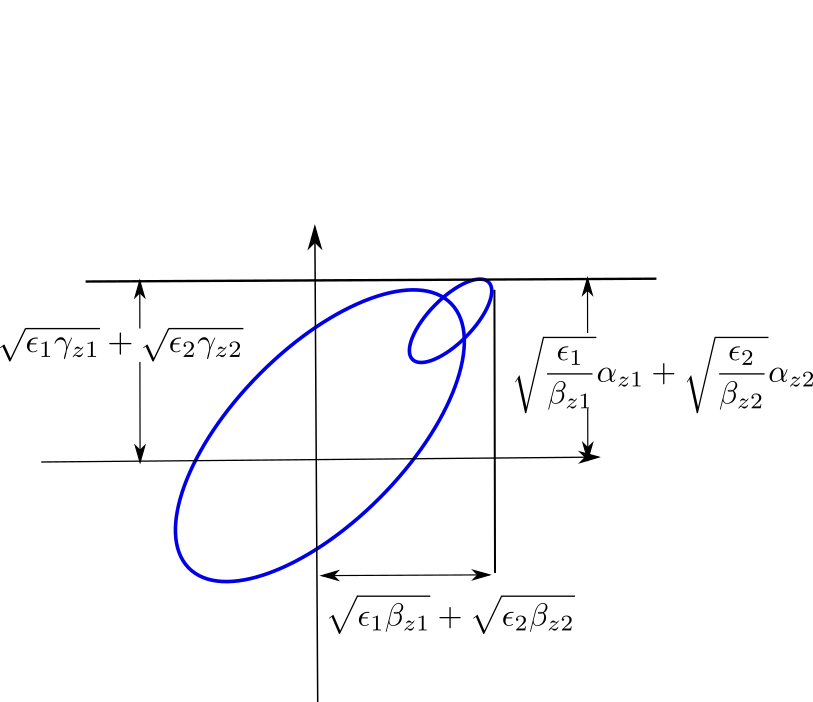
\includegraphics[width=1.0\linewidth]{ripken_phase_space_ellipse.png}
	\caption{Projection of lattice function in the $z-z'$ plane.\label{opt:fig:2}}
\end{figure}

Using Eqns.~\ref{opt:eqn:3:3}, \ref{opt:eqn:4:1}, \ref{opt:eqn:4:2} and $\cos(x+y)=\cos x\cos y-\sin x\sin y$, the coordinates $z(s)$ can be expressed by:
\begin{align}
z_{2j-1}(s)&=\sum_{k=1}^3 \sqrt{2I_k
\beta_{k,j}(s)}\cos{(\phi_{k,j}(s)+\phi_{k,0})}\\
z_{2j}(s)&=\sum_{k=1}^3 \sqrt{2I_k
\gamma_{k,j}(s)}\cos{(\bar\phi_{k,j}(s)+\phi_{k,0})}, \ j=1,\ldots,3
\end{align}
Conversely the lattice functions can also be expressed by $a_k$ and $b_k$ with
\begin{align}
\beta_{k,j}(s)&=a_{k,2j-1}(s)^2 +b_{k,2j-1}(s)^2 \\
\alpha_{k,j}(s)&=a_{k,2j-1}(s)a_{k,2j}(s) -b_{k,2j-1}(s)b_{k,2j}(s) \\
\gamma_{k,j}(s)&=a_{k,2j}(s)^2 +b_{k,2j}(s)^2,
\end{align}
The well known relations between the lattice functions
\begin{align}
\sum_{j=1}^3\beta_{k,j}\phi_{k,j}'&=1 \\
\gamma_{k,j}&=\frac{\beta_{k,j}^2\phi_{k,j}'^2+\alpha_{k,j}^2}{\beta_{k,j}}, \text{ with  }\\
\alpha_{k,j}&:=-\frac{1}{2}\beta_{k,j}'
\end{align}
can then be derived with the help of the normalization condition (Eqn.~\ref{opt:eqn:2:3})
\begin{align}
a_k^TSb_k=1
\end{align}
by the following steps:
\begin{enumerate}
\item As $x'=\frac{dx}{ds},\ y'=\frac{dy}{ds}$ and $\delta=\frac{d\sigma}{ds}$ the following relations hold also for $a_k$ and $b_k$:
\begin{align}
a_{k,2j}=a_{k,2j-1}'&=\frac{d}{ds}(a_{k,2j-1}), \\
b_{k,2j}=b_{k,2j-1}'&=\frac{d}{ds}(b_{k,2j-1}),\ k,j=1,\ldots,3 
\end{align}
\item The normalization condition Eqn.~\ref{opt:eqn:2:3} can then be written as
\begin{align}
a_k^TSb_k&=\sum_{j=1}^3\sqrt{\beta_{k,j}}\cos{\phi_{k,j}}\left(\sqrt{\beta_{k,j}}\sin{\phi_{k,j}}\right)'\nonumber\\
& \qquad -\left(\sqrt{\beta_{k,j}}\cos{\phi_{k,j}}\right)'\sqrt{\beta_{k,j}}\sin{\phi_{k,j}}\nonumber\\
&=\sum_{j=1}^3\beta_{k,j}\phi_{k,j}'\nonumber\\
&=1 \label{opt:eqn:4:3}
\end{align}
Note that Eqn.~\ref{opt:eqn:4:3} yields the the following relation between the phase advance $\phi$ and $\beta$ in 2D:
\begin{align}
\phi(s)=\phi(0)+\int_{s_0}^s\frac{1}{\beta(\bar s)}d\bar s
\end{align}
\item Using the abbreviation $\alpha_{k,j}:=-\frac{1}{2}\beta_{k,j}$, one finds for each mode $k$ and plane $j$
\begin{align}
\sqrt{\gamma_{k,j}}\cos{\phi_{k,j}}&=a_{k,2j}=a_{k,2j-1}'=(\sqrt{\beta_{k,j}}\cos{\phi_{k,j}})' &\quad (1)\nonumber\\
\sqrt{\gamma_{k,j}}\sin{\phi_{k,j}}&=b_{k,2j}=b_{k,2j-1}'=(\sqrt{\beta_{k,j}}\sin{\phi_{k,j}})' &\quad (2)\nonumber\\
\overset{(1)^2+(2)^2}{\Rightarrow} \gamma_{k,j}&=\frac{\beta_{k,j}^2\phi_{k,j}'^2+\alpha_{k,j}^2}{\beta_{k,j}}, \quad k,j=1,\ldots,3 &
\end{align}
which simplifies in the 2D case to:
\begin{align}
\gamma\overset{\rm Eqn.~\ref{opt:eqn:4:3}}{=}\frac{1+\alpha^2}{\beta}
\end{align}
\end{enumerate}

\section{Notation}

\begin{description}
\item $\vec R$: moving reference frame origin
\item $s$: path length of the reference frame origin trajectory
\item $\hat X, \hat Y,\hat Z$: global coordinate bases
\item $X, Y, Z$: reference frame origin coordinates $\vec R(s)=X(s) \hat X+Y(s) \hat Y+ Z(s) \hat Z$
\item $T$ Absolute time in the global frame
\item $\hat x(s), \hat y(s), \hat s(s)$: moving reference frame bases
\item $\vec Q$: particle position
\item $x, y$: transverse particle coordinates $\vec Q(s)= \vec R(s) + x(s) \,\hat x(s) + y(s)\, \hat y(s)$
\item $t(s)$: time at which the particle is located in the plane $\hat x(s), \hat y(s)$
\item $v, P, E, m, q$: particle velocity momenta, energy, rest mass, charge
\item $v_0, P_0, E_0, m_0, q_0$ Reference momentum, energy, rest mass,
\item $\beta, \gamma$: PArticle relativistic factors
\item $\beta_0, \gamma_0$: Reference relativistic factors
\item $\tau=s/\beta_0 - c t$: Mad time deviation, canonical conjugate of $p_\tau$
\item $\sigma=s - \beta_0 c t$: SixTrack time deviation, canonical conjugate of $p_\sigma$
\item $\Delta s=s - \beta c t  $  path length deviation, canonical conjugate of $\delta$
\item $z=\beta(s/\beta_0 - c t) $  John Jowet's time deviation, canonical conjugate of $\delta$
\item $P_x, P_y,  P_s$: canonical momenta coordinates in a straight or curved reference frame. Note that for a planar curvilinear trajectory in a electromagnetic field.
$P_s=m \gamma \dot s (1 + hx)^2 + q (1 + hx) A_s$ and $v_s= (1 +h x) \dot s$ where $h=1\rho$ is the inverse of the curvature in the s,x plane.   
\item $p_x=P_x/P_0, p_y=P_x/P_0, p_s=P_s/P_0$ normalized conamical momenta coordinates
\item $x'=P_x/P_s,y'=P_x/P_s$ transverse divergence coordinates
\item $x_p=P_x/P,y_p=P_y/P$ approximate divergence coordinates
\item $\delta=(P-P_0)/P_0$: momentum deviation
\item $p_\tau=(E-E_0)/P_0c$: energy deviation
\item $p_\sigma=(E-E_0)/(\beta_0 P_0c)$: SixTrack energy deviation canonical conjugate of $\sigma$
\item $H$ Hamiltonian function
\item $E_x, E_y, E_s$ Electric fields in a straight or curved reference frame
\item $B_x, B_y, B_s$ Magnetic fluxes in a straight or curved reference frame
\item $A_x, A_y, A_s$ Magnetic fluxes in a straight or curved reference frame
\end{description}


\bibliographystyle{unsrt}
\bibliography{bibliography}


\end{document}
